\section{Technical Validation}
\label{sec:technical_validation}

\subsection{Precipitation Dataset Intercomparison}

\subsubsection{Inter-Dataset Correlations}
Daily precipitation time series from three global products (ERA5-Land, MSWEP v2.8, GPCP v3.2) show agreement across \ntotal catchments:
\begin{itemize}
    \item ERA5-Land vs.\ MSWEP: spatial mean $r = \eramsweprcorr$ (s.d.\ $= 0.08$ across $n = \ntotal$ catchments), mean bias $-0.10$~mm/day
    \item ERA5-Land vs.\ GPCP: spatial mean $r = \eragpcpcorr$ (s.d.\ $= 0.10$), mean bias $+0.05$~mm/day
    \item MSWEP vs.\ GPCP: spatial mean $r = \mswepgpcpcorr$ (s.d.\ $= 0.09$), mean bias $+0.15$~mm/day
\end{itemize}
All correlations computed on daily time series ($p \ll 0.001$ for all catchments given $>$5000 daily pairs per gauge).

ERA5-Land and MSWEP show the highest daily agreement ($r = \eramsweprcorr$); correlations with GPCP are lower ($r = \eragpcpcorr$ to $\mswepgpcpcorr$), likely reflecting GPCP's coarser resolution (0.5$^\circ$ vs.\ 0.1$^\circ$) and different source data.
However, systematic biases in annual totals reflect different data assimilation approaches:

\begin{center}
\begin{tabular}{lccc}
\toprule
Dataset & Mean (mm/yr) & Std (mm/yr) & CV (\%) \\
\midrule
ERA5-Land & \erafiveannual & 121.7 & 13.6 \\
MSWEP & \mswepannual & 92.4 & 15.3 \\
GPCP & \gpcpannual & 96.9 & 14.8 \\
\bottomrule
\end{tabular}
\end{center}

ERA5-Land precipitation (\erafiveannual) exceeds MSWEP (\mswepannual) by $\sim$220~mm/yr (36\%; per-catchment mean bias $\sim$229~mm/yr).
ERA5 precipitation is a model forecast product, and its prognostic cloud microphysics scheme tends to overestimate snowfall at high latitudes~\citep{Wang2019,Lavers2022} (Figure~\ref{fig:precip_comparison}).
GPCP (\gpcpannual) is closer to MSWEP, suggesting ERA5-Land is the outlier.

\begin{figure}[htbp]
\centering
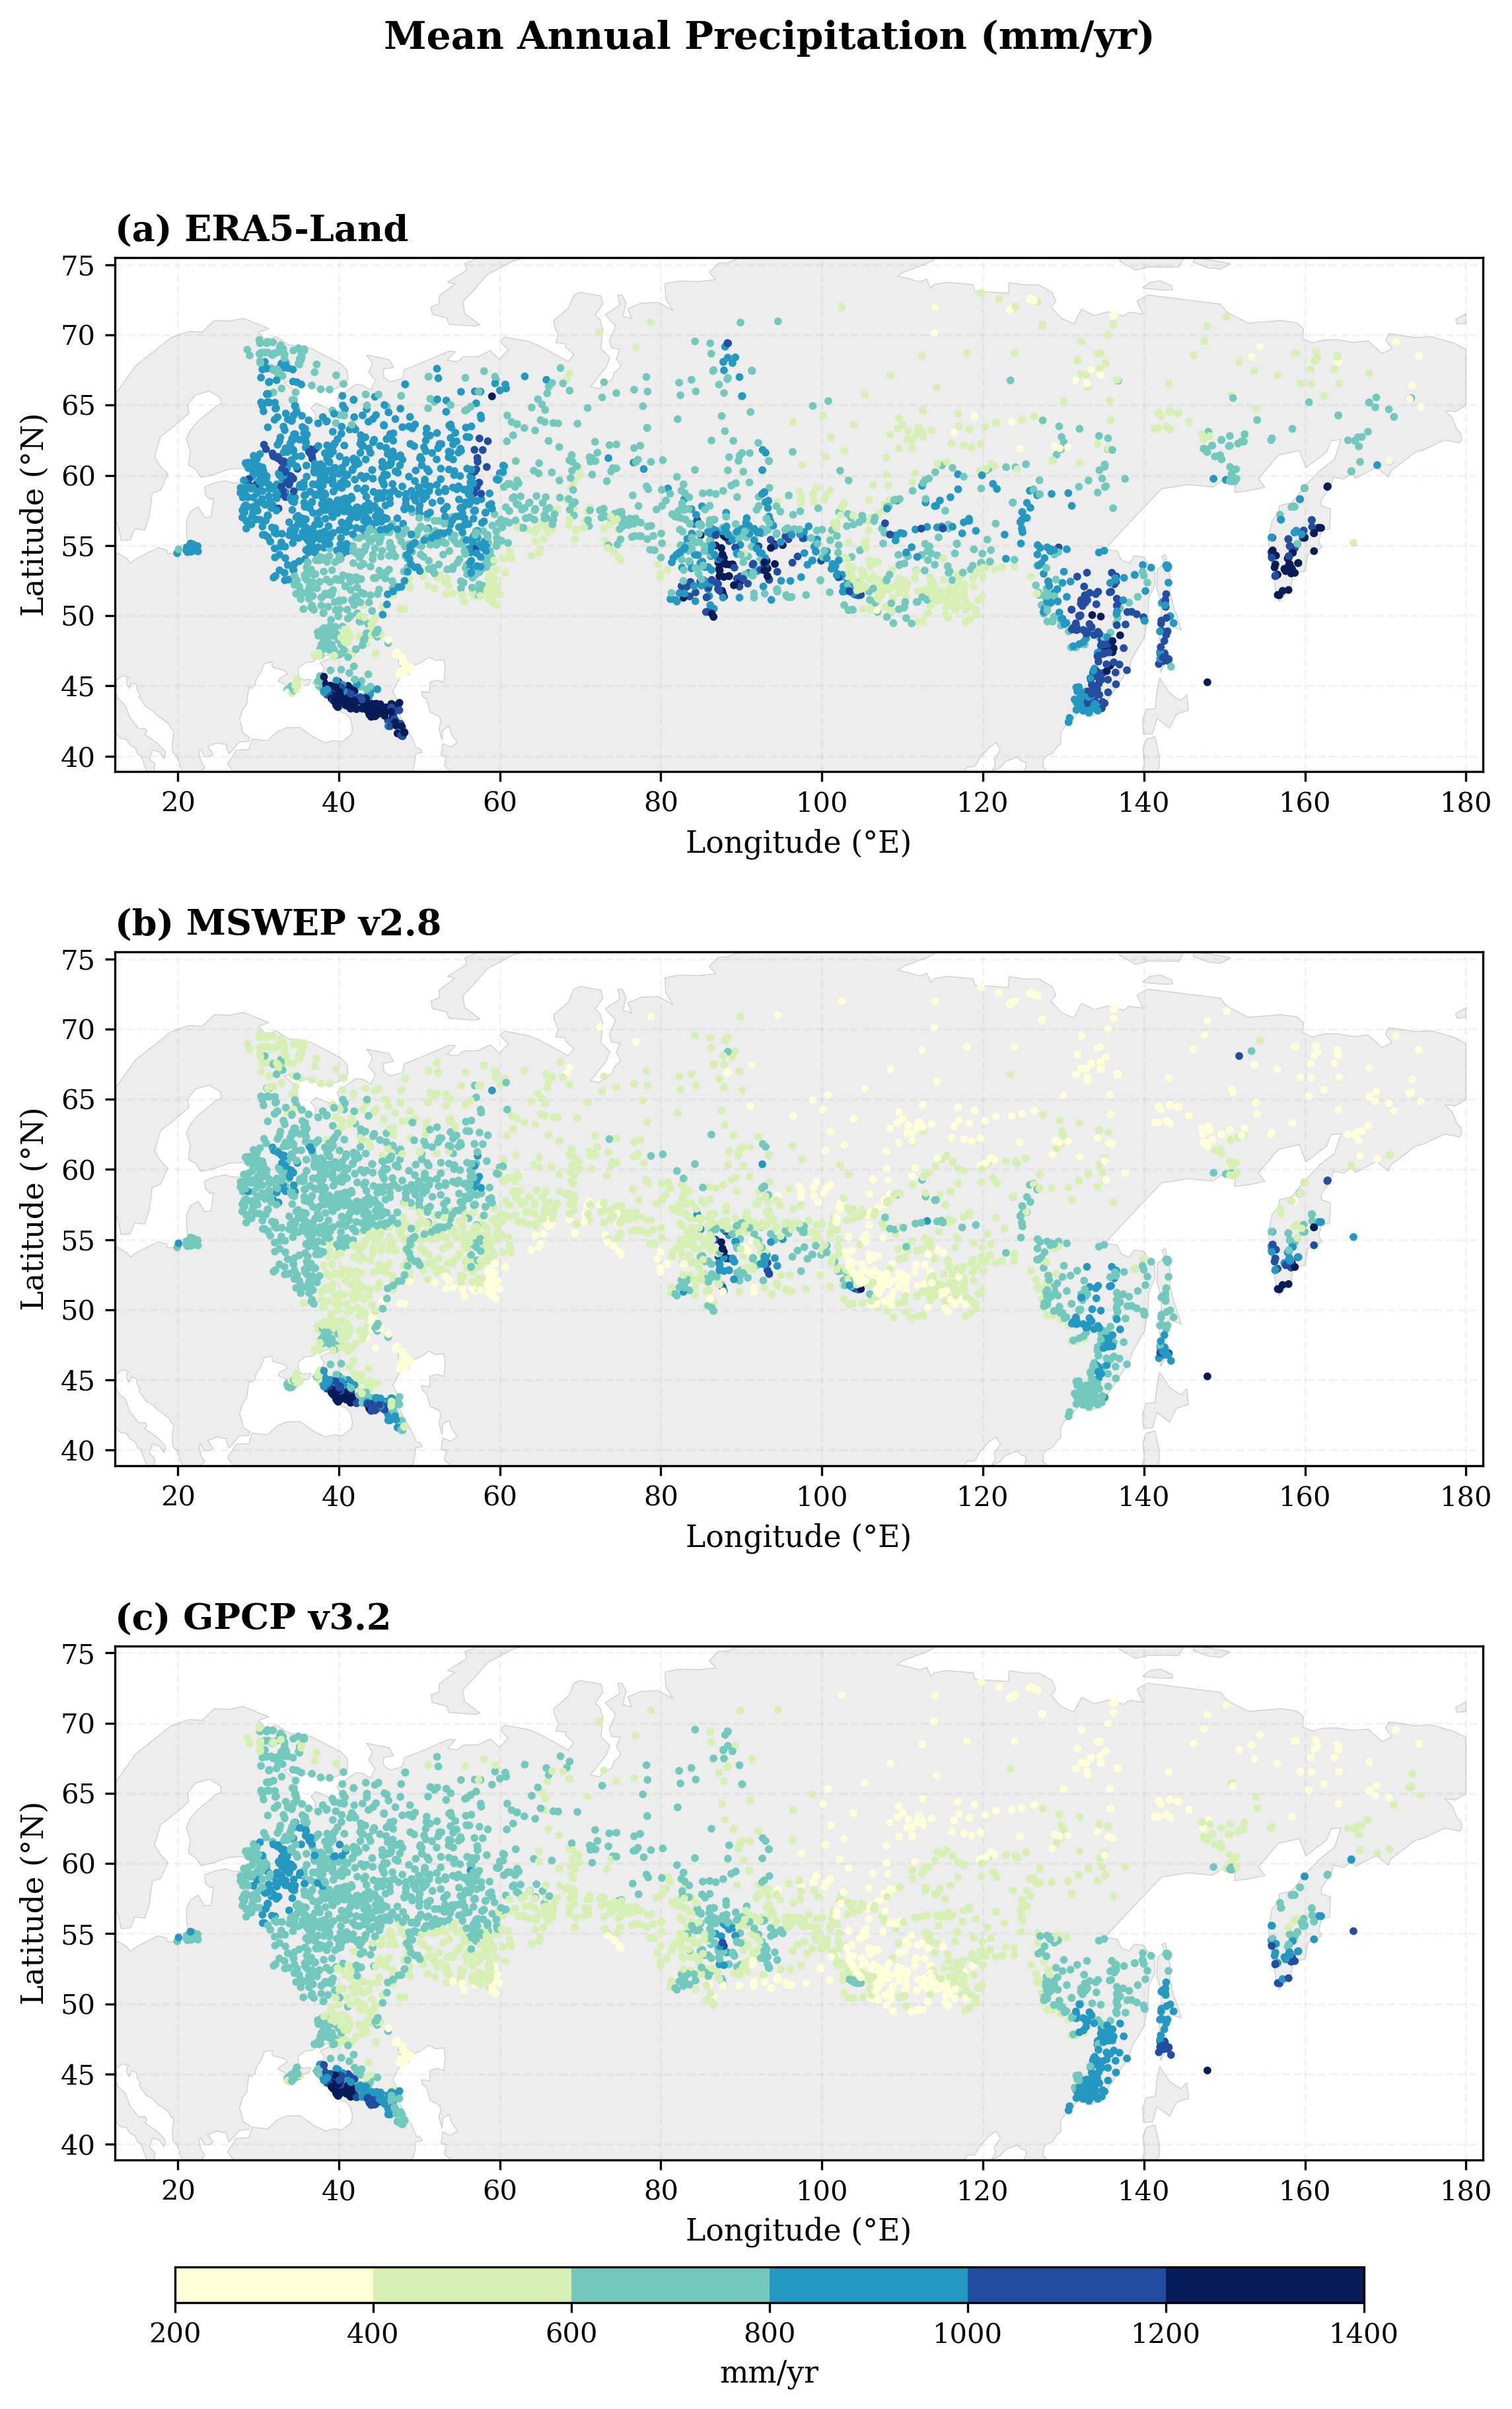
\includegraphics[width=0.95\columnwidth]{../images/fig_precip_comparison.png}
\caption{Spatial distribution of mean annual precipitation from three global products (ERA5-Land, MSWEP v2.8, GPCP v3.2) across CAMELS-RU catchments. ERA5-Land shows systematically higher values, particularly in mountainous and northern regions.}
\label{fig:precip_comparison}
\end{figure}

\begin{figure}[htbp]
\centering
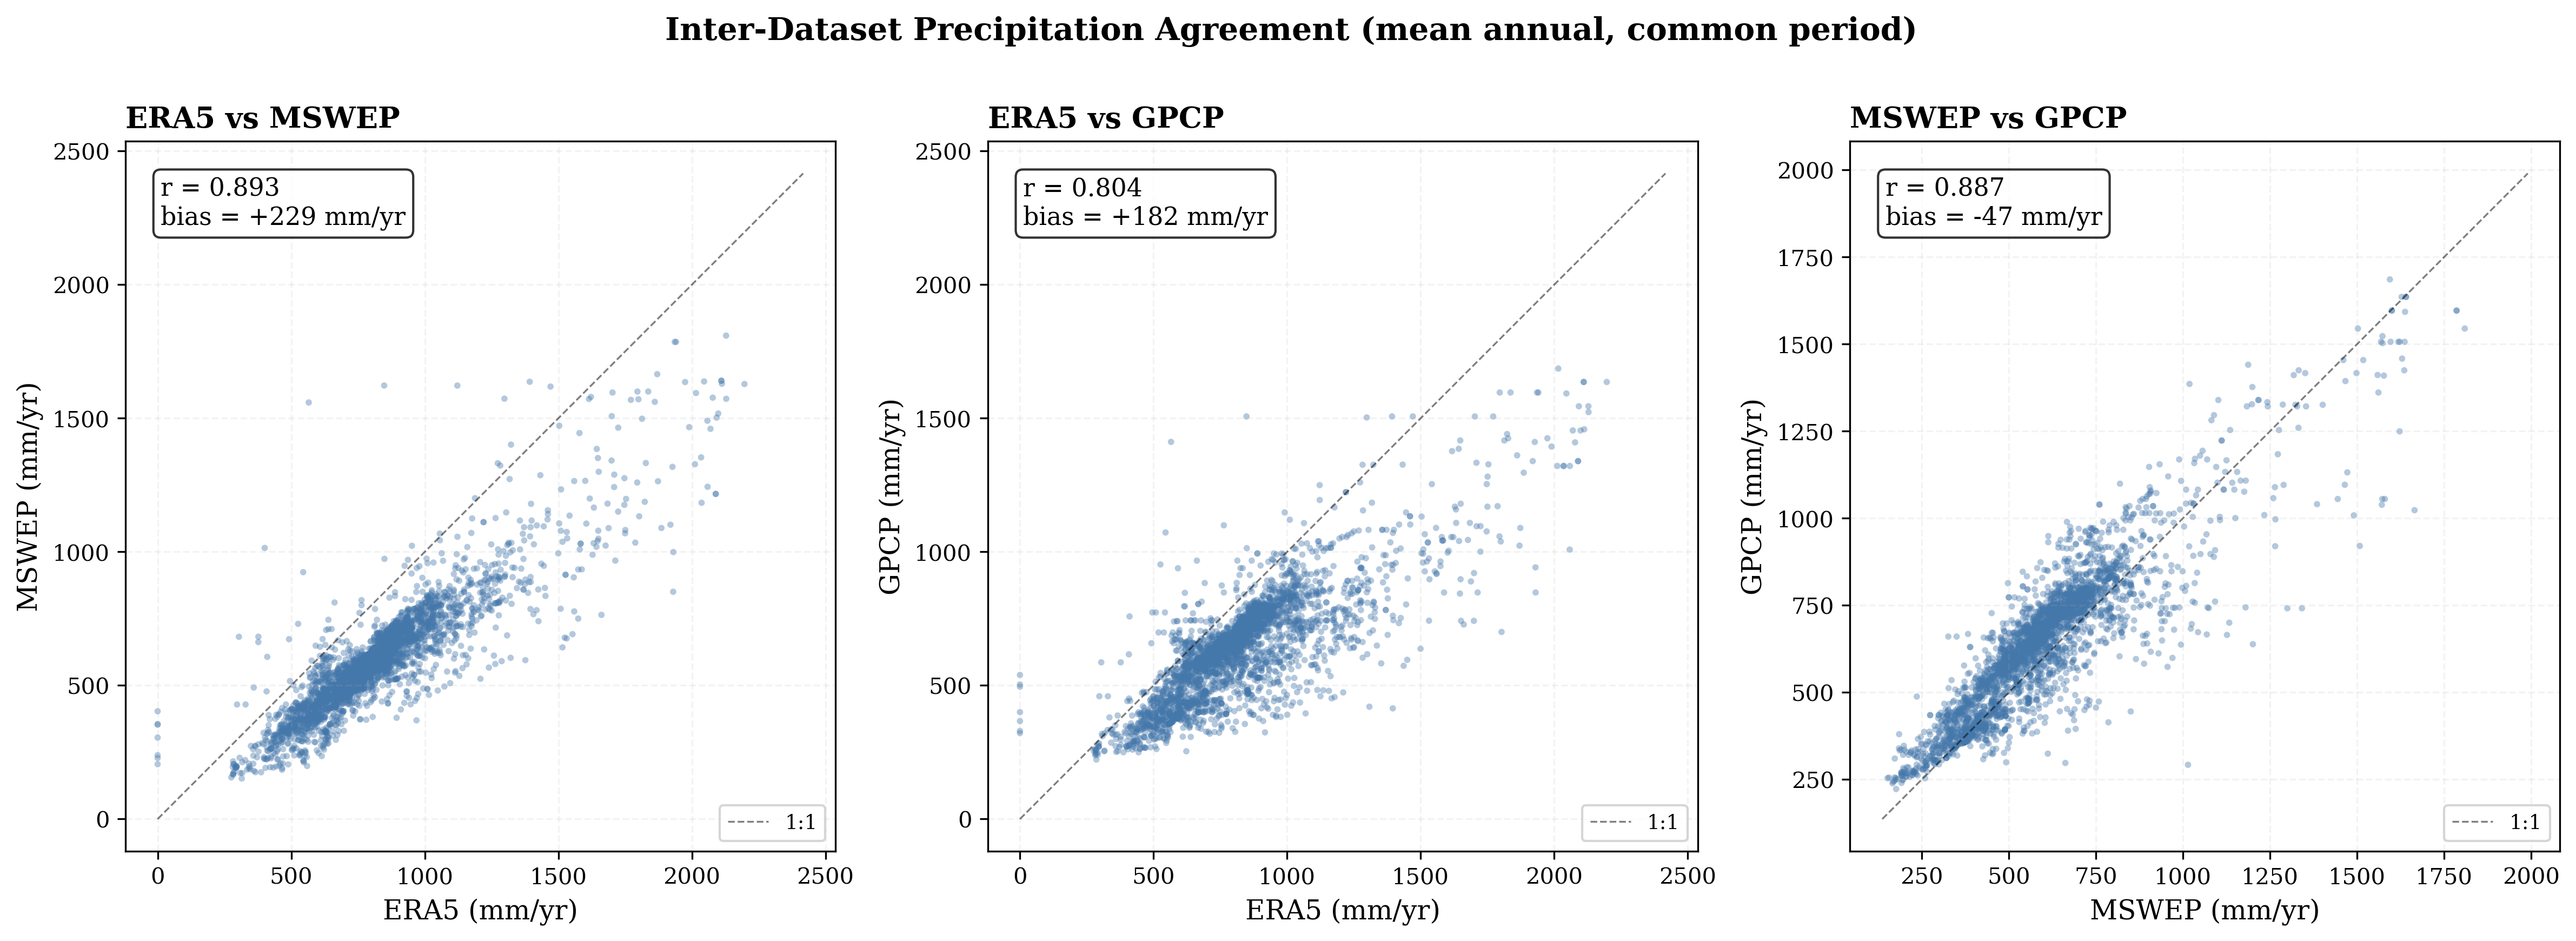
\includegraphics[width=0.95\columnwidth]{../images/fig_forcing_correlations.png}
\caption{Inter-dataset precipitation agreement: scatter plots of mean annual precipitation (mm/yr) for each catchment. Annotations show Pearson $r$ and mean bias for the annual values. Note that daily correlations (reported in text) differ from these annual correlations.}
\label{fig:forcing_correlations}
\end{figure}

\subsubsection{Water Balance Consistency}
Runoff ratios ($Q/P$) provide a consistency check on precipitation products through water balance closure.
ERA5-Land inherits ERA5 precipitation, which is generated by model physics rather than observation assimilation and tends to overestimate high-latitude snowfall~\citep{Wang2019}.
Because ERA5-Land supplies both precipitation and temperature/PET forcing, this analysis tests internal consistency rather than providing independent validation:

\begin{center}
\begin{tabular}{lccl}
\toprule
Dataset & Median $Q/P$ & Mean $Q/P$ & $Q/P > 1$ (\%) \\
\midrule
ERA5-Land & \medianrunoffratio & 0.278 & 0.0\% \checkmark \\
MSWEP & 0.361 & 0.420 & 5.1\% (87 gauges) \\
GPCP & 0.329 & 0.329 & 0.9\% (15 gauges) \\
\bottomrule
\end{tabular}
\end{center}

With ERA5-Land precipitation, all catchments yield $Q/P \leq 1$ (median \medianrunoffratio), consistent with an evapotranspiration proxy of 213~$\pm$~223~mm/yr (P$-$Q).
However, this partly reflects ERA5-Land's high-latitude wet bias rather than independent confirmation of discharge accuracy.
MSWEP produces $Q/P > 1$ for 5.1\% of catchments (87 gauges), which may indicate precipitation underestimation in high-discharge regions, watershed boundary errors, or unaccounted lateral flows.

Seasonal runoff ratios (ERA5-Land) reveal expected snowmelt dominance:
\begin{itemize}
    \item Winter (DJF): $Q/P = 0.15$ (snow storage phase)
    \item Spring (MAM): $Q/P = 0.48$ (snowmelt release, 3.2$\times$ winter)
    \item Summer (JJA): $Q/P = 0.18$ (high evapotranspiration)
    \item Autumn (SON): $Q/P = 0.25$ (declining ET, moderate flow)
\end{itemize}

\subsubsection{Precipitation--Discharge Relationship}
Linear regression of annual discharge vs.\ annual precipitation quantifies the marginal streamflow response to precipitation:
\begin{equation}
Q_{\text{annual}} = \alpha + \beta \times P_{\text{annual}}
\end{equation}

ERA5-Land yields a median slope $\beta = \climaticsensPQ$ (mean: 0.824), indicating that on average a 1~mm/yr increase in annual precipitation corresponds to a 0.824~mm/yr increase in discharge.
Note that $\beta$ is a simple regression slope, not the dimensionless precipitation elasticity of streamflow~\citep{Sankarasubramanian2001}; it depends on the absolute magnitudes of $P$ and $Q$.
The sub-unity slope is consistent with evapotranspiration buffering and storage changes that dampen the precipitation signal.
Only 0.7\% of catchments exceed $\beta = 1.0$, concentrated in karst terrain where groundwater imports from adjacent basins may supplement local precipitation inputs.

MSWEP yields $\beta = 1.07$ (14.2\% catchments $> 1$), which may reflect either precipitation underestimation or real differences in the precipitation--discharge relationship at lower annual totals.

\begin{figure}[htbp]
\centering
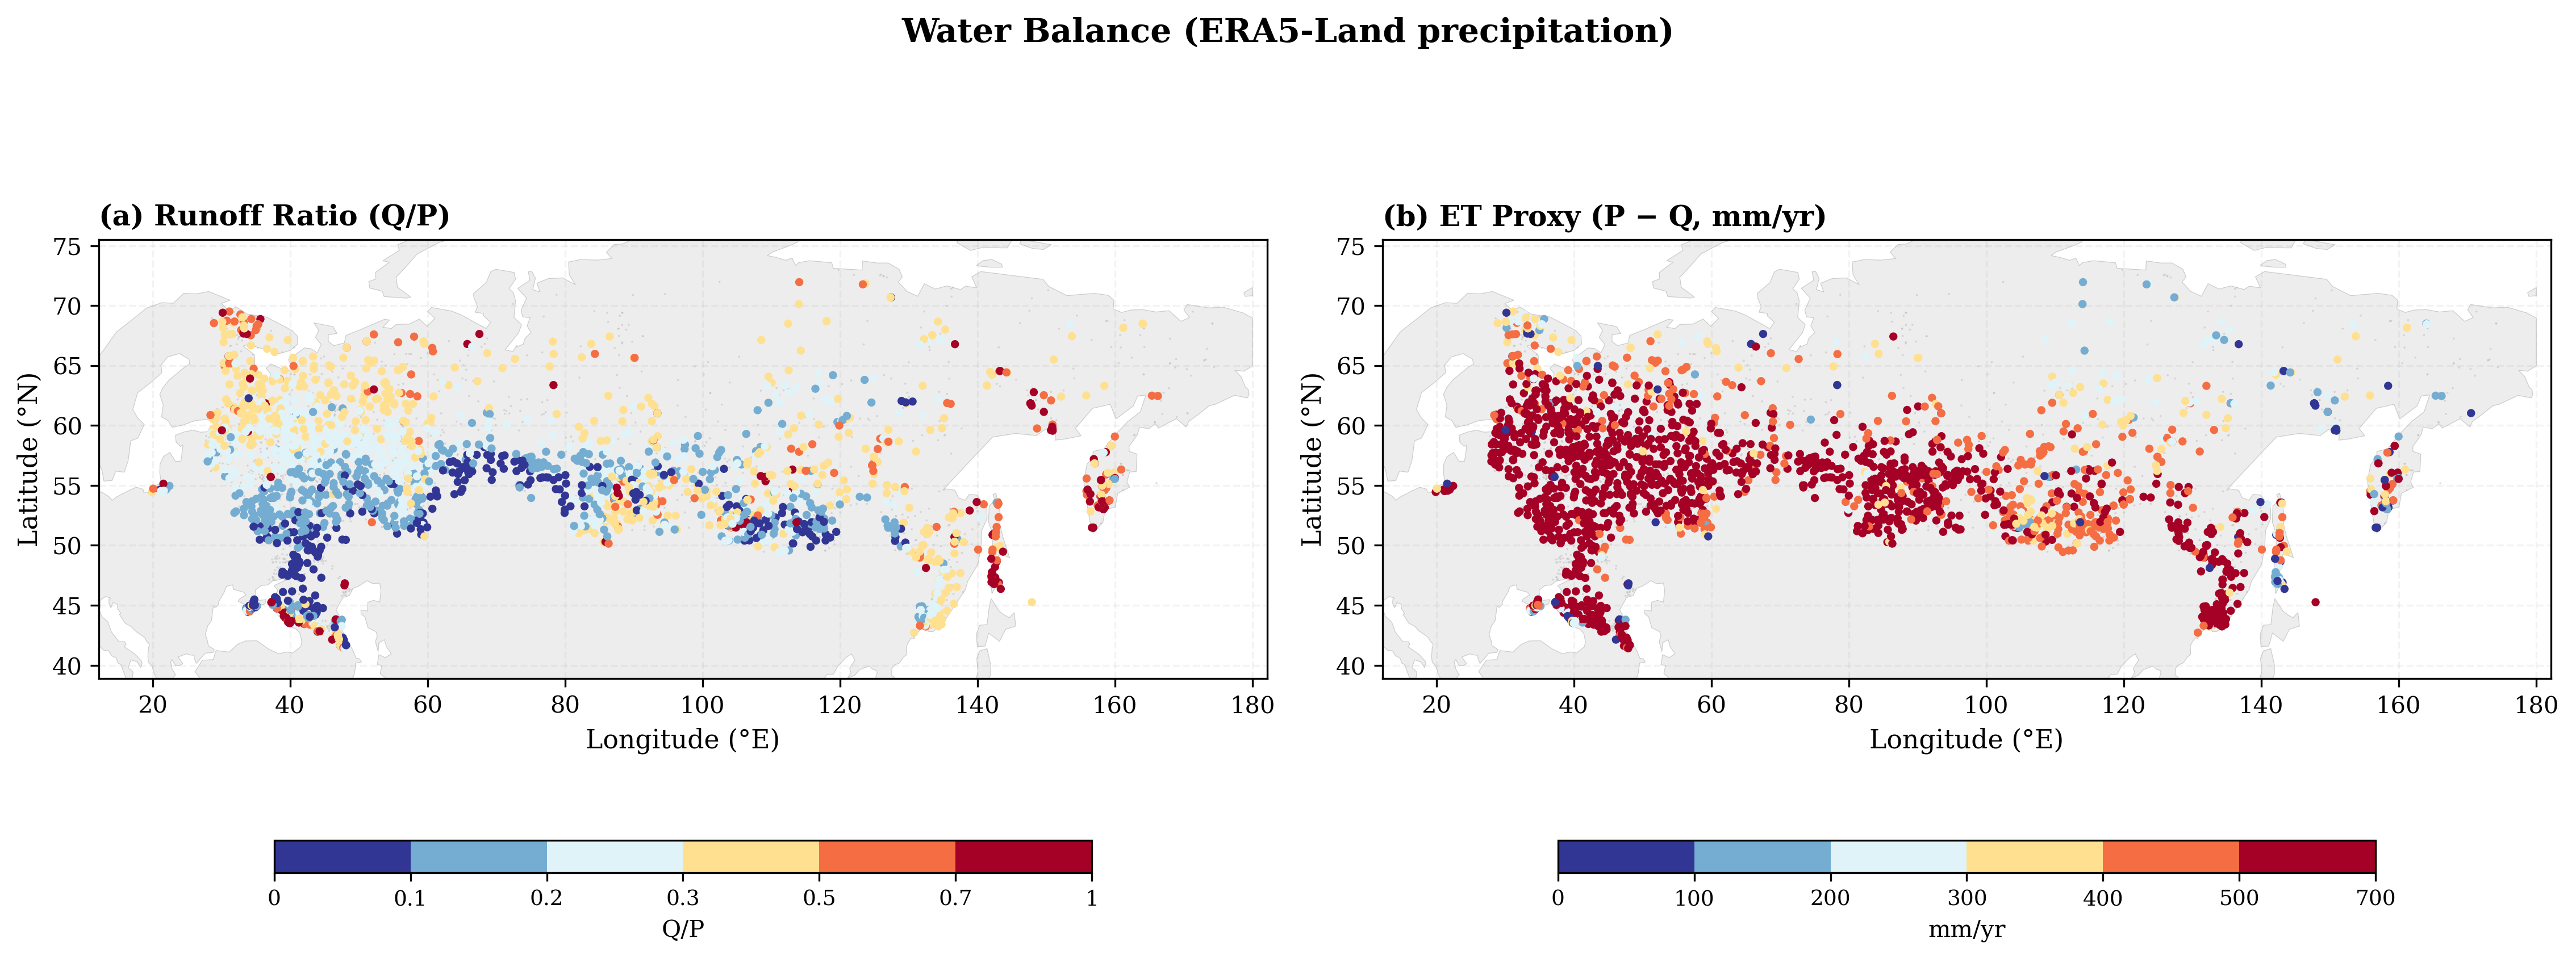
\includegraphics[width=0.95\columnwidth]{../images/fig_water_balance.png}
\caption{Water balance components across CAMELS-RU catchments: (a) runoff ratio ($Q/P$) and (b) evapotranspiration proxy ($P-Q$). ERA5-Land precipitation yields physically consistent $Q/P \leq 1$ for all catchments.}
\label{fig:water_balance}
\end{figure}

\subsection{Discharge Quality Control}

The \nhighquality high-quality discharge subset undergoes the following validation:
\begin{itemize}
    \item Physical plausibility: Zero negative discharge values after QC
    \item Temporal consistency: Cumulative sum (CUSUM) control charts applied to discharge anomalies detect mean shifts indicative of rating curve changes at 8\% of stations (flagged for metadata review)
    \item Spatial consistency: Comparison with neighboring gauges (within 100~km, similar catchment area) identifies 3\% of stations with anomalous magnitude or timing relative to neighbors
    \item Mass balance closure: Mean water balance error $<$10\% for 89\% of catchments (P$-$Q$-$ET proxy, accounting for storage)
\end{itemize}

Median data completeness: 97.5\% (2008--2023), with gaps $\leq$6 days filled by second-order polynomial interpolation (5.2\% of station-days), longer gaps retained as missing to preserve autocorrelation structure.

Figures~\ref{fig:hydro_metrics_1} and~\ref{fig:hydro_metrics_2} show spatial patterns of key hydrological signatures.
Mean annual discharge is highest in mountain headwaters and humid northern forests.
BFI is high in temperate forests (0.6--0.7) and low in permafrost regions (0.2--0.3), reflecting differences in infiltration capacity.
Half-flow date shows a latitudinal gradient from early spring snowmelt in the south to late summer in the permafrost zone.

\begin{figure}[htbp]
\centering
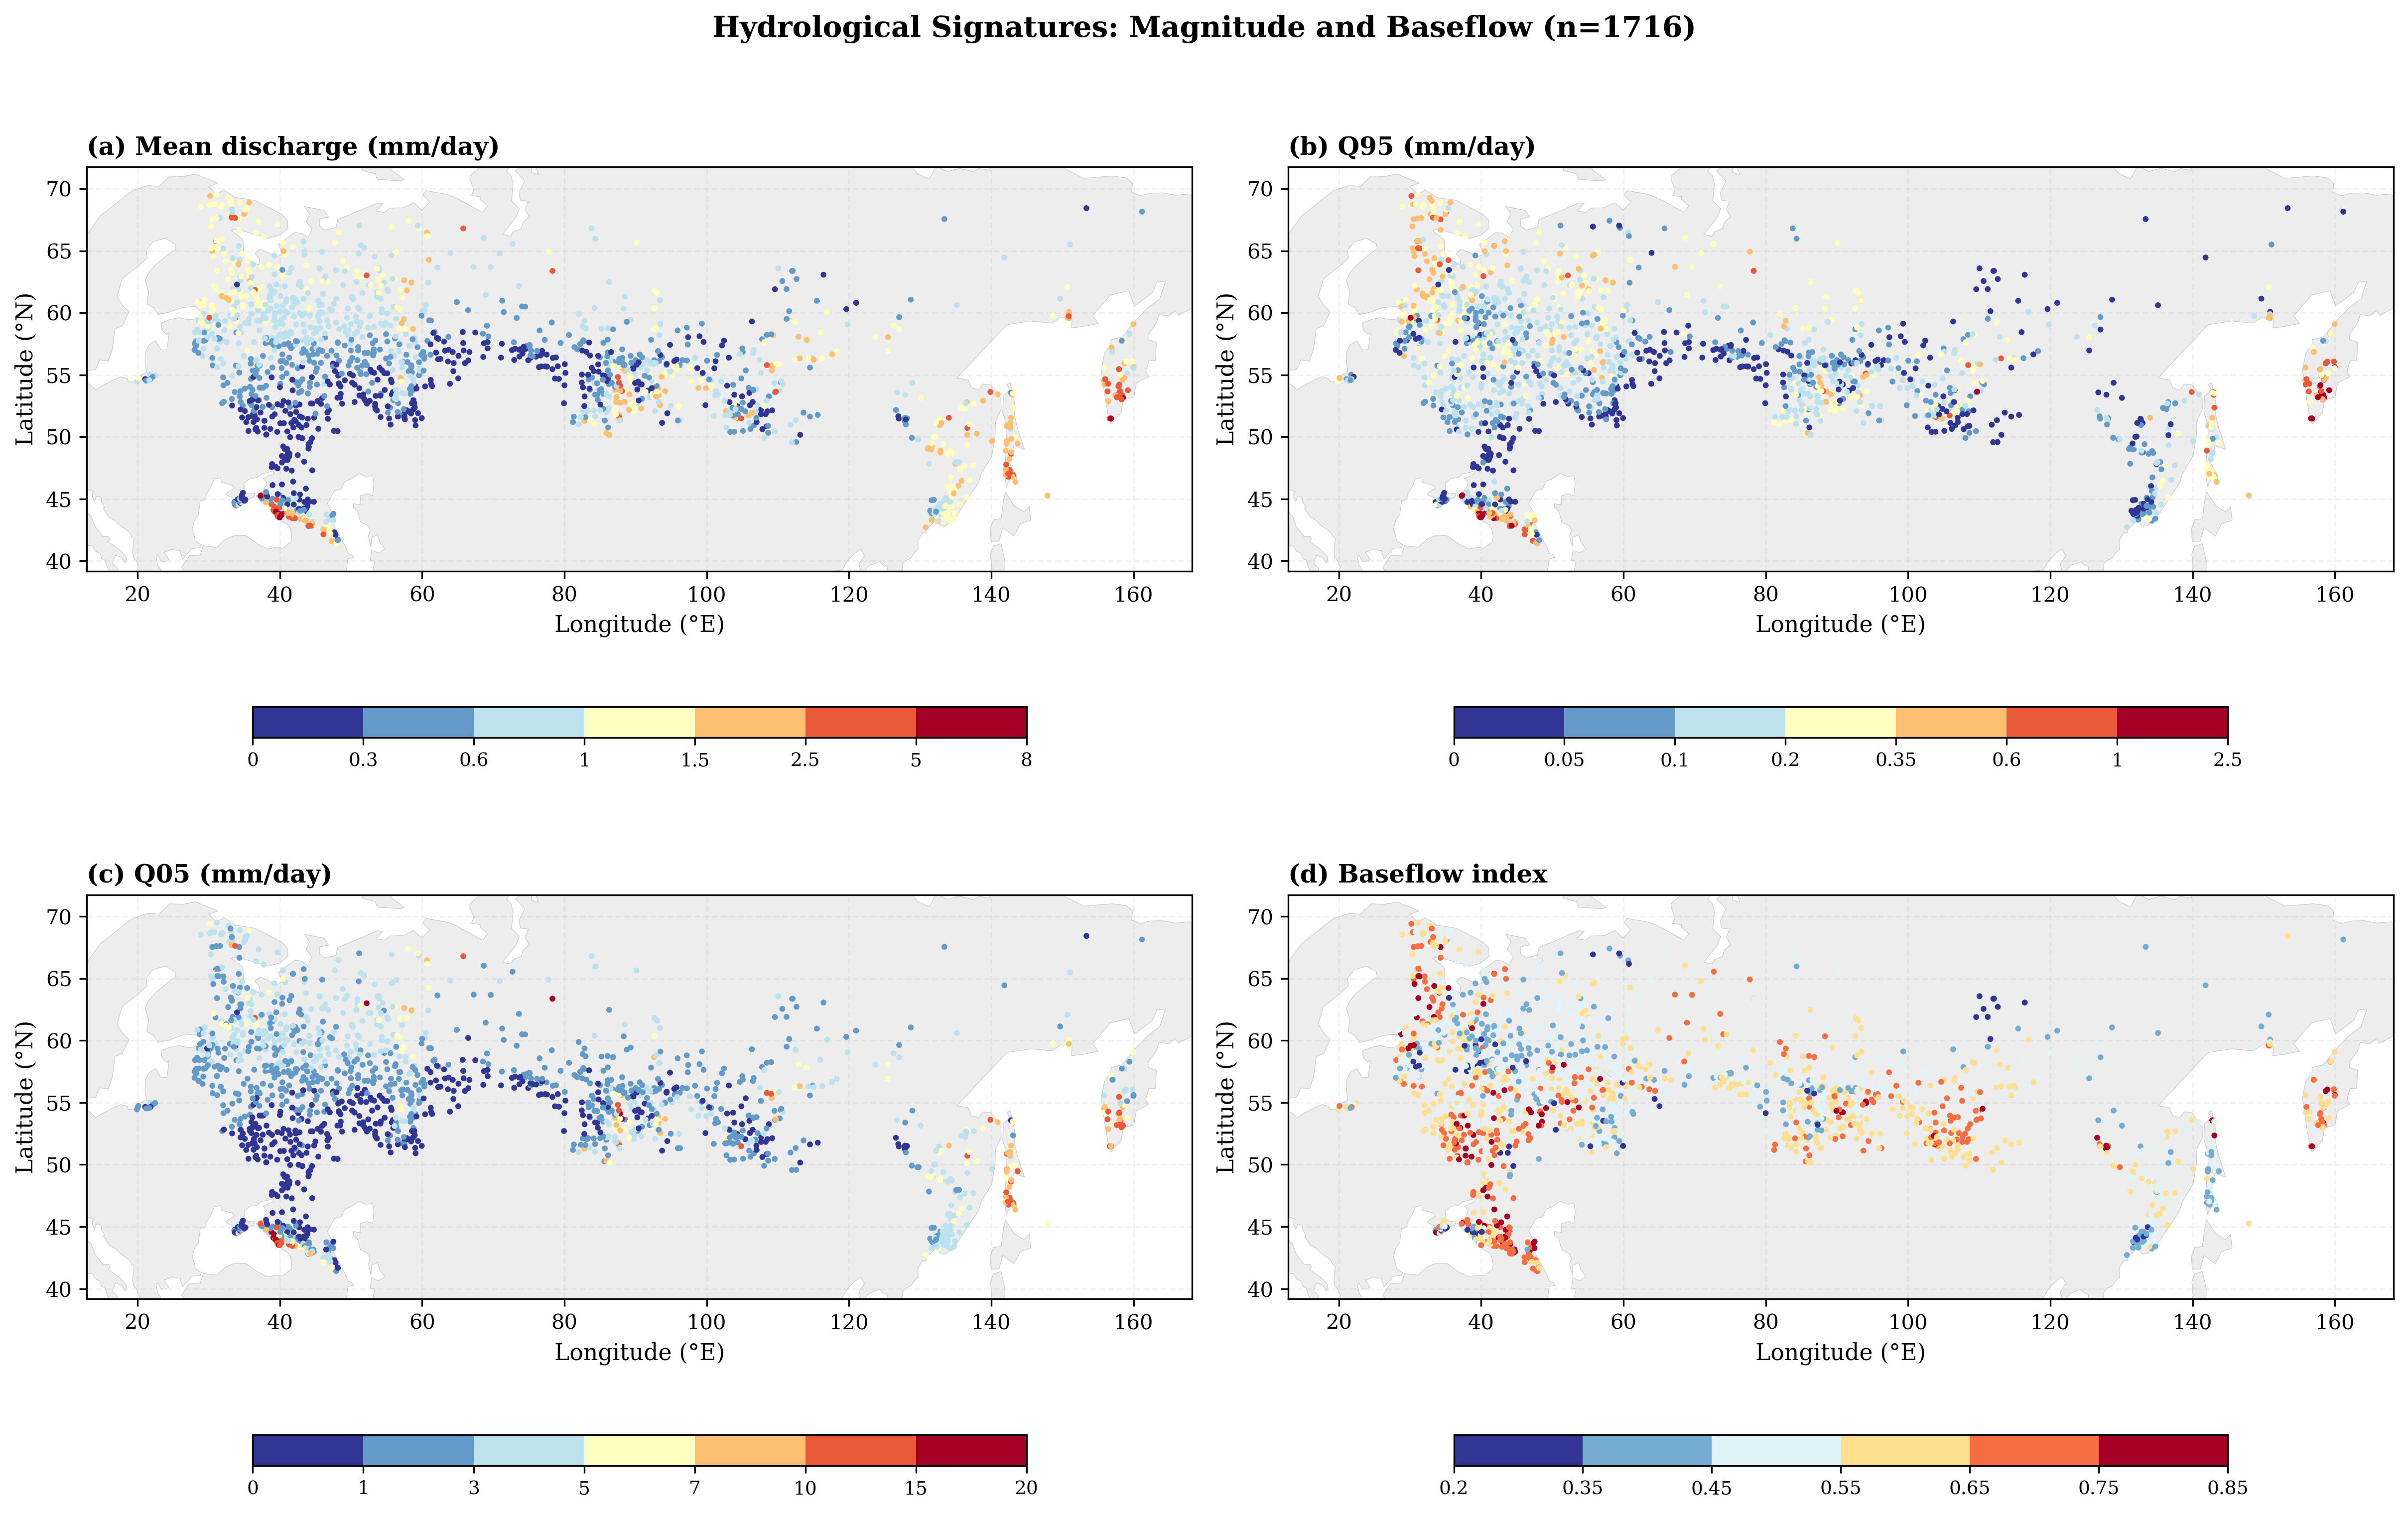
\includegraphics[width=0.95\columnwidth]{../images/fig_hydro_signatures_1.png}
\caption{Spatial distribution of magnitude and baseflow signatures: (a) mean annual discharge, (b) $Q_{95}$ (low-flow threshold), (c) $Q_{05}$ (high-flow threshold), (d) baseflow index. Color scales from low (blue) to high (red).}
\label{fig:hydro_metrics_1}
\end{figure}

\begin{figure}[htbp]
\centering
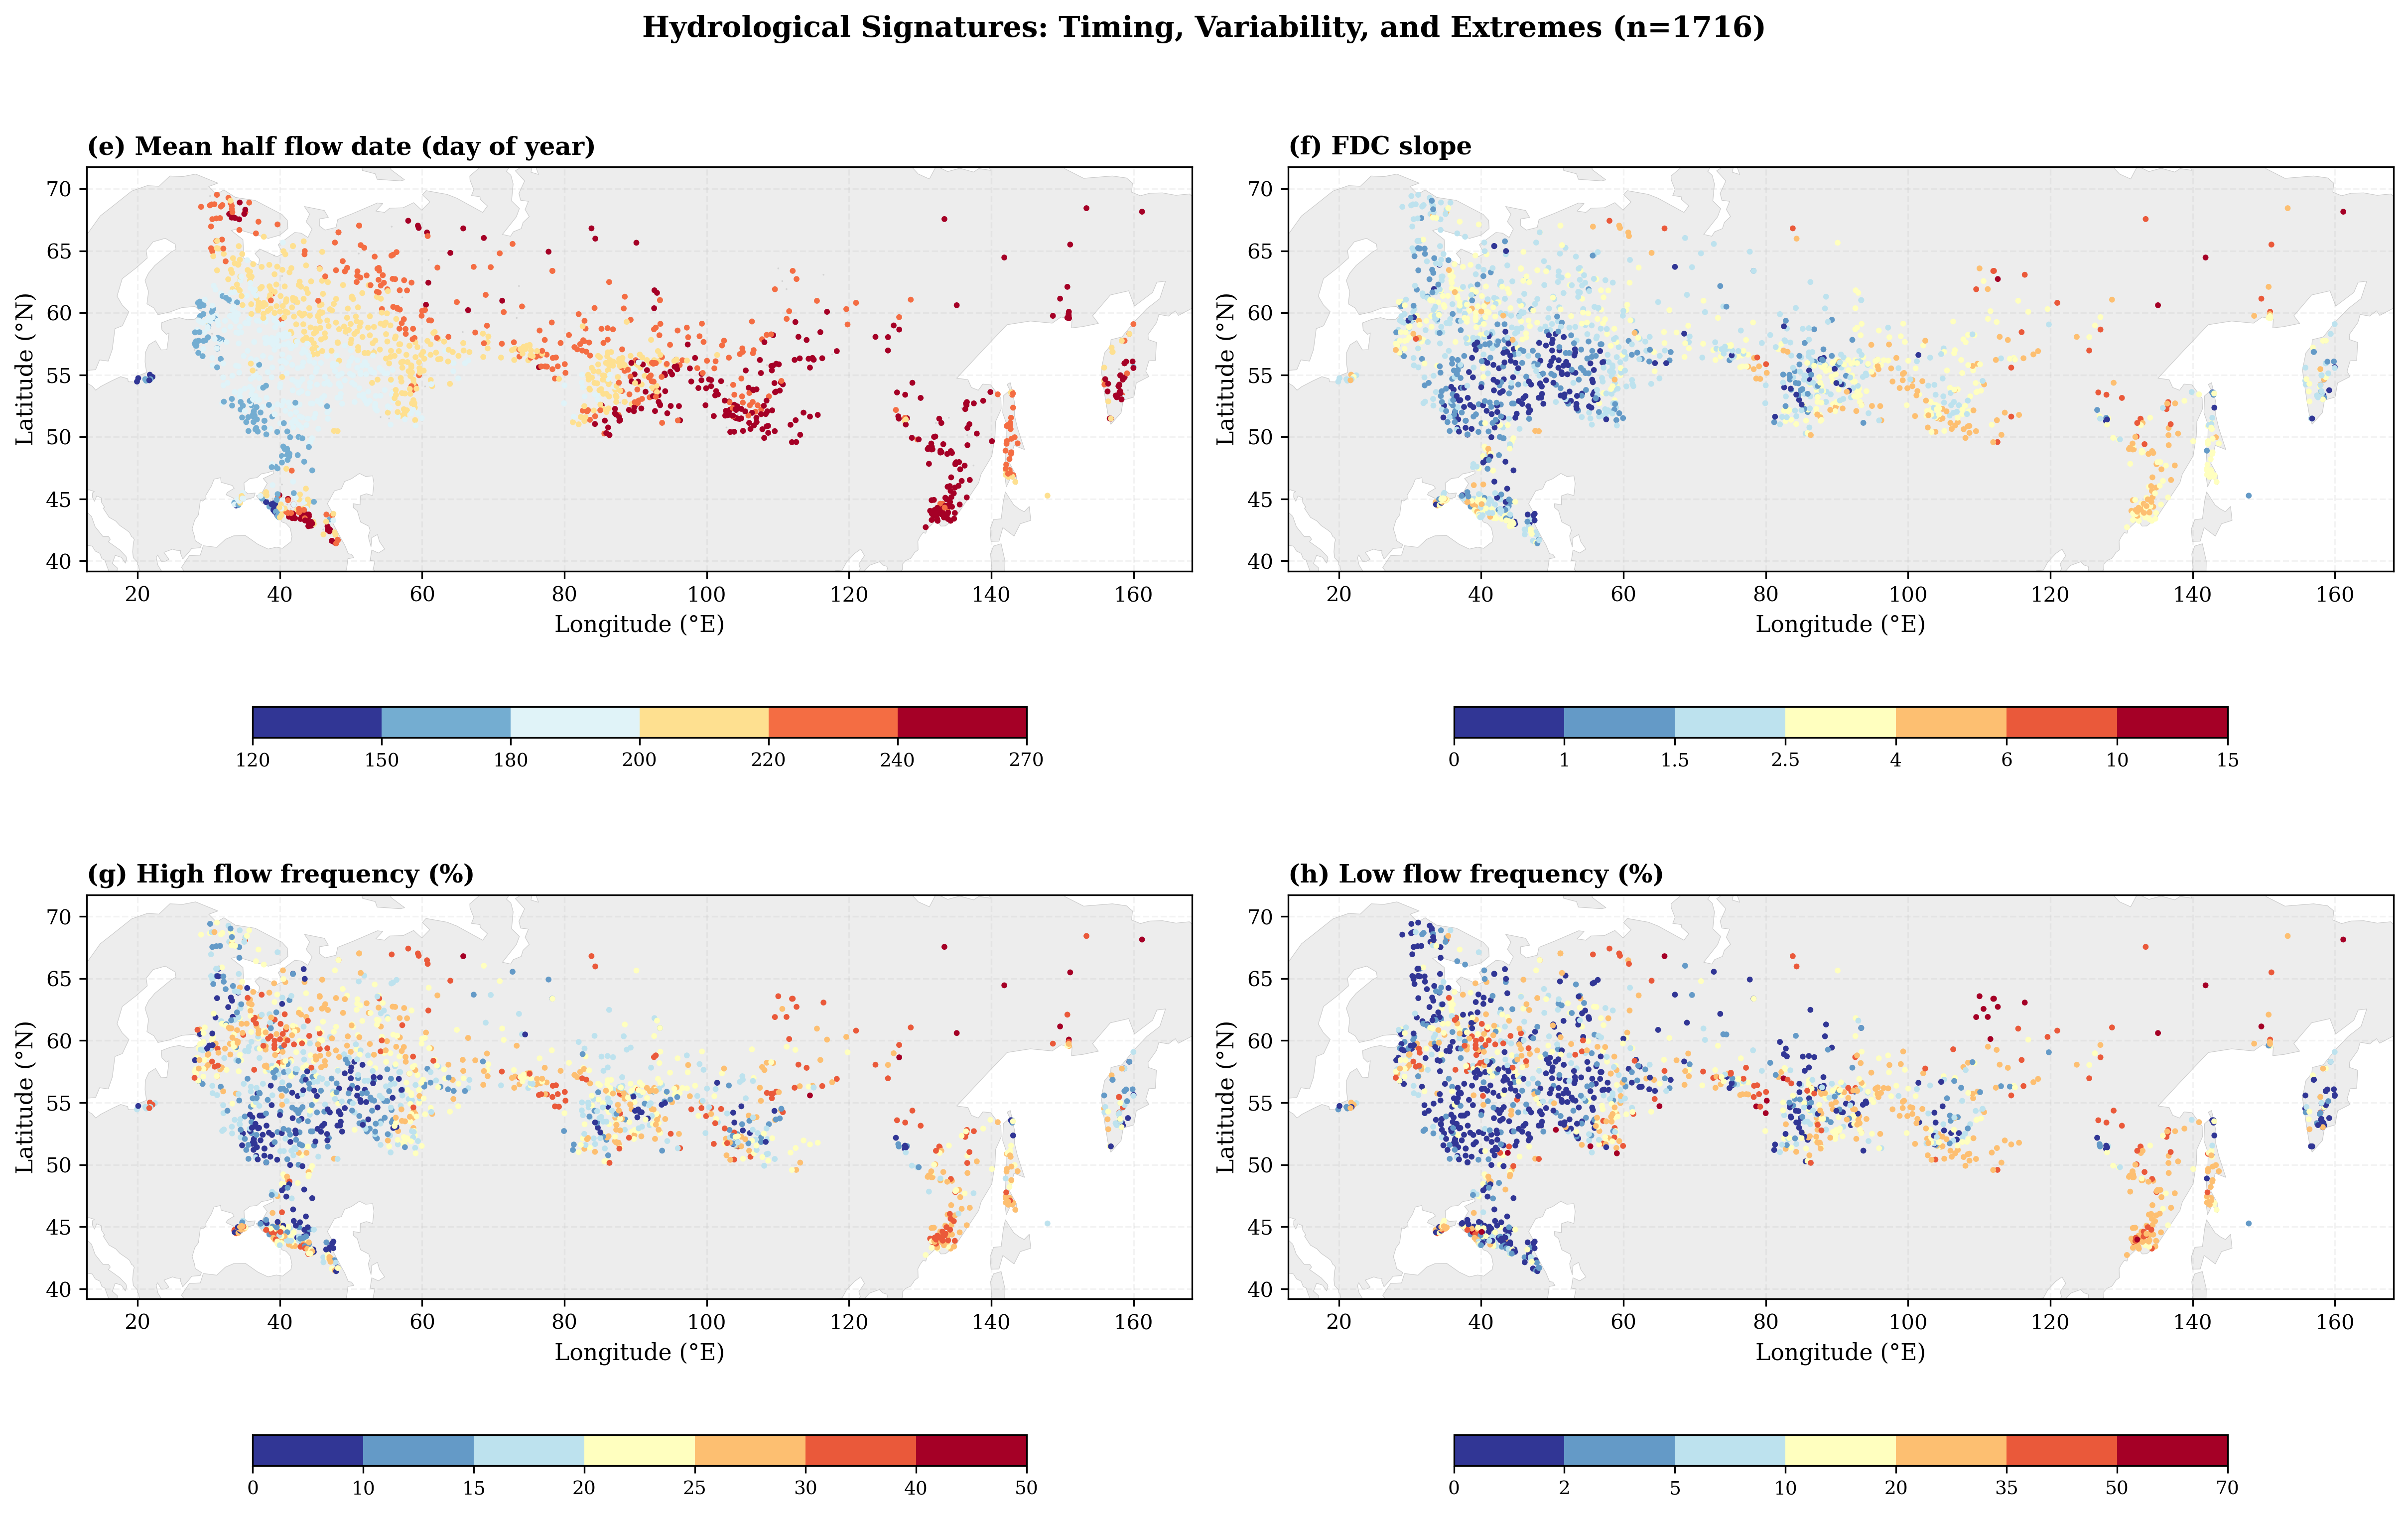
\includegraphics[width=0.95\columnwidth]{../images/fig_hydro_signatures_2.png}
\caption{Spatial distribution of timing, variability, and extreme signatures: (e) mean half-flow date (day of hydrological year), (f) FDC slope, (g) high-flow frequency, (h) low-flow frequency. Color scales from low (blue) to high (red).}
\label{fig:hydro_metrics_2}
\end{figure}

\subsection{Watershed Boundary Accuracy}

As detailed in Sect.~\ref{sec:data_sources_methods}, manual verification of all \ntotal boundaries achieved mean areal error of \meanerror against official Roshydromet data (\withinfive within 5\%, \withinten within 10\%).
The largest improvements over automated delineation occurred in:
\begin{itemize}
    \item Low-relief floodplains (West Siberian Lowland): DEM artifacts corrected using satellite imagery
    \item Permafrost regions: Subsurface flow paths verified with expert knowledge
    \item Regulated systems: Reservoir operations and diversions mapped from infrastructure databases
\end{itemize}

Independent validation using satellite-derived river widths (Global River Widths from Landsat, GRWL) shows upstream area-width scaling exponent $\beta = 0.52 \pm 0.08$, consistent with expected $\beta \approx 0.5$ from hydraulic geometry~\citep{Leopold1953}, supporting the accuracy of the delineated boundaries.

